\documentclass[a4paper,12pt]{article} % добавить leqno в [] для нумерации слева
\usepackage[a4paper,top=1.3cm,bottom=2cm,left=1.5cm,right=1.5cm,marginparwidth=0.75cm]{geometry}

\usepackage[warn]{mathtext}
\usepackage[T2A]{fontenc}
\usepackage[utf8]{inputenc} 
\usepackage[english, russian]{babel}

\usepackage{ upgreek }
\usepackage[table,xcdraw]{xcolor}

\usepackage{indentfirst} %tabutation

\usepackage{amsmath, amsfonts, amssymb, amsthm, mathtools, mathtext} 

\usepackage{graphicx}

\usepackage{wrapfig}
\usepackage{tabularx}

\usepackage{graphicx}%Вставка картинок правильная
\usepackage{float}%"Плавающие" картинки
\usepackage{wrapfig}% Обтекание фигур (таблиц, картинок и прочего)

%%% Дополнительная работа с математикой
\usepackage{amsmath,amsfonts,amssymb,amsthm,mathtools} % AMS





%%% Заголовок
\author{Устюжанина Мария Алексеевна}
\title{Лабораторная работа №1.2.3
Отчет о выполнении лабораторной работы 1.2.
}
\date{\today}

\begin{document}

\begin{titlepage}
	\begin{center}
		{\large МОСКОВСКИЙ ФИЗИКО-ТЕХНИЧЕСКИЙ ИНСТИТУТ (НАЦИОНАЛЬНЫЙ ИССЛЕДОВАТЕЛЬСКИЙ УНИВЕРСИТЕТ)}
	\end{center}
	\begin{center}
		{\large Физтех-школа радиотехники и компьютерных технологий}
	\end{center}
	
	
	\vspace{4.5cm}
	{\huge
		\begin{center}
			{\bf Лабораторная работа № 2.1.6}\\
			 Эффект Джоуля-Томстона.
		\end{center}
	}
	\vspace{4cm}
	\begin{flushright}
		{\LARGE Автор:\\ Устюжанина Мария Алексеевна \\
			\vspace{0.3cm}
			Б01-107}
	\end{flushright}
	\vspace{6cm}
	\begin{center}
		Долгопрудный 2022
	\end{center}
\end{titlepage}

\section{Введение}

\textbf{Цель работы:}

1) Определение изменения температуры углекислого газа при протекании через малопроницаемую перегородку при разных начальных значениях дав- ления и температуры; 

2) Вычисление по результатам опытов коэффициен- тов Ван дер Ваальса «a» и «b».

\

\textbf{Используемое оборудование:}
Трубка с пористой перегородкой; труба Дьюара; термостат; термометры; дифференциальная термопара; микровольтметр; балластный баллон; ма- нометр.

\section{Выполнение работы и результаты}

\begin{enumerate}

	 Проведем измерения температуры с помощью вольтметра при разном давлении меняя температуру.

	\item Результаты измерений и график при комнатной температуре:

$$
\begin{tabular}{|c|c|c|c|c|c|}
\hline
\multicolumn{6}{|c|}{При $T = 296 K$}\\
\hline
$\Delta P, Pa$&4&3.5&3.2&2.7&2.1\\\hline
$\Delta T, K$& 5.291& 4.558& 3.826& 3.053& 2.035\\\hline
\end{tabular}
$$


\begin{figure}[h]
	\center{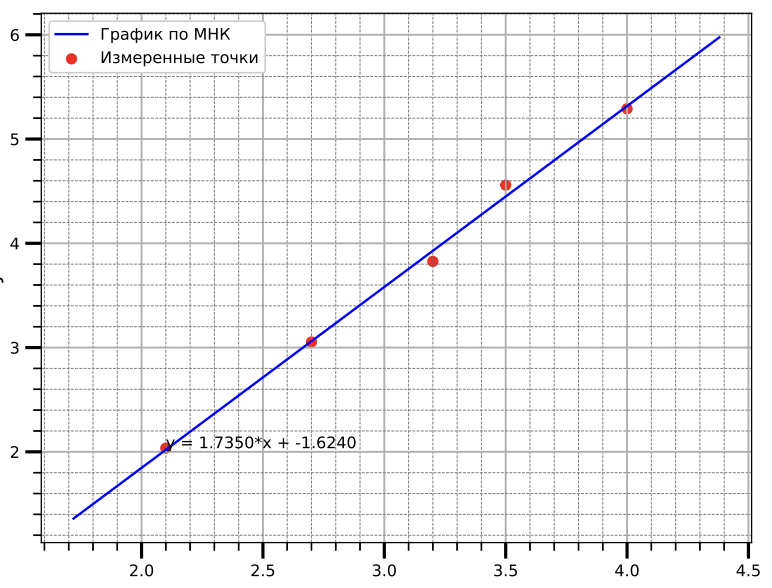
\includegraphics[width=400]{Graf1}}
	\caption{Зависимость $ \delta T / \delta P $ \ при \ T = 296 K}
\end{figure}

Получилась зависимость: 


\[ \frac{\delta T}{\delta P} = 1.7 \pm 0.5 \ \frac{K}{Па}\]

\medskip



\\\\\\\\\\\\\\\\\\\\\\\\\\\\\\\\\\\\\\\\\\\\\\\\\\\\\\\\\\\\\\\\




	\itemРезультаты измерений и график при температуре 303К:


$$
\begin{tabular}{|c|c|c|c|c|c|}
\hline
\multicolumn{6}{|c|}{При $T = 303 K$}\\
\hline
$\Delta P, Pa$&4.0&3.5&3.3&2.7&2.2\\\hline
$\Delta T, K$& 5.088& 4.192& 3.866& 2.768& 1.994\\\hline
\end{tabular}
$$


\begin{figure}[h]
	\center{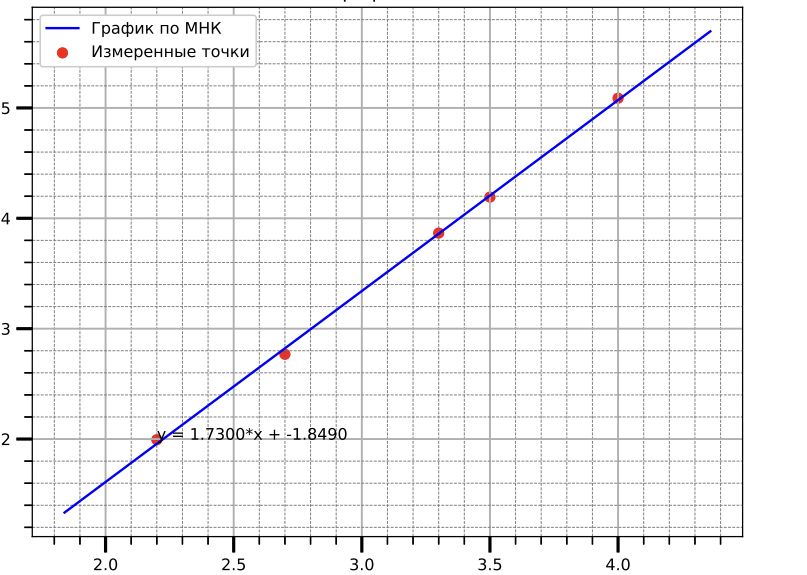
\includegraphics[width=400]{Graf2}}
	\caption{Зависимость $ \delta T / \delta P $ \ при \ T = 303 K}
\end{figure}

Получилась зависимость: 


\[ \frac{\delta T}{\delta P} = 1.7 \pm 0.5 \ \frac{K}{Па}\]

\medskip





\\\\\\\\\\\\\\\\\\\\\\\\\\\\\\\\\\\\\\\\\\\\\\\\\\\\\\\\\\

\item Результаты измерений и график при температуре 313К:

$$
\begin{tabular}{|c|c|c|c|c|c|}
\hline
\multicolumn{6}{|c|}{При $T = 313 K$}\\
\hline
$\Delta P, Pa$&4.1&3.5&3.2&2.7&2.2\\\hline
$\Delta T, K$& 4.95& 3.952& 3.411& 2.87& 1.955\\\hline
\end{tabular}
$$


\begin{figure}[h]
	\center{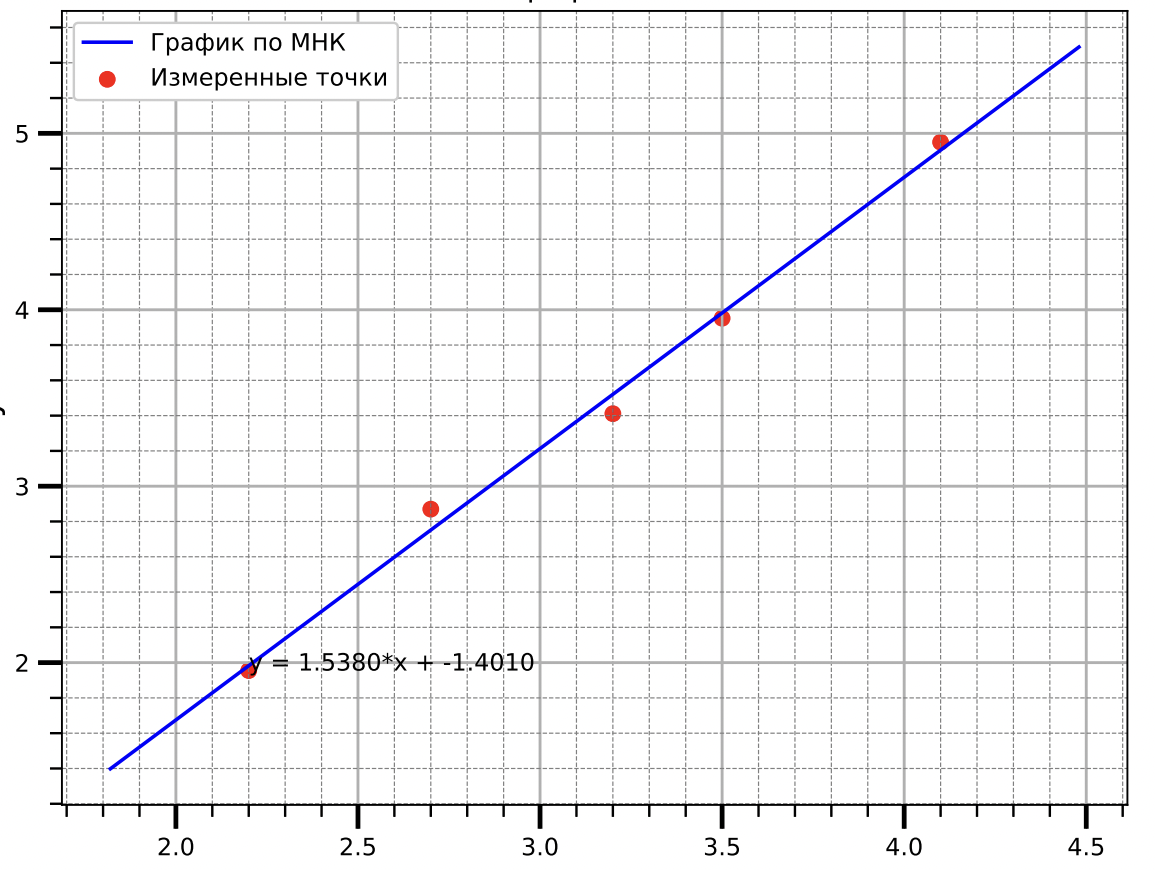
\includegraphics[width=400]{Graf3}}
	\caption{Зависимость $ \delta T / \delta P $ \ при \ T = 313 K}
\end{figure}

Получилась зависимость: 


\[ \frac{\delta T}{\delta P} = 1.5 \pm 0.5 \ \frac{K}{Па}\]

\medskip





\\\\\\\\\\\\\\\\\\\\\\\\\\\\\\\\\\\\\\\\\\\\\\\\\\\\\\



\item Результаты измерений и график при температуре 323К:

$$
\begin{tabular}{|c|c|c|c|c|c|}
\hline
\multicolumn{6}{|c|}{При $T = 323 K$}\\
\hline
$\Delta P, Pa$&4.1&3.5&3.2&2.7&2.2\\\hline
$\Delta T, K$& 4.8& 3.825& 3.442& 2.72& 1.955\\\hline
\end{tabular}
$$


\begin{figure}[h]
	\center{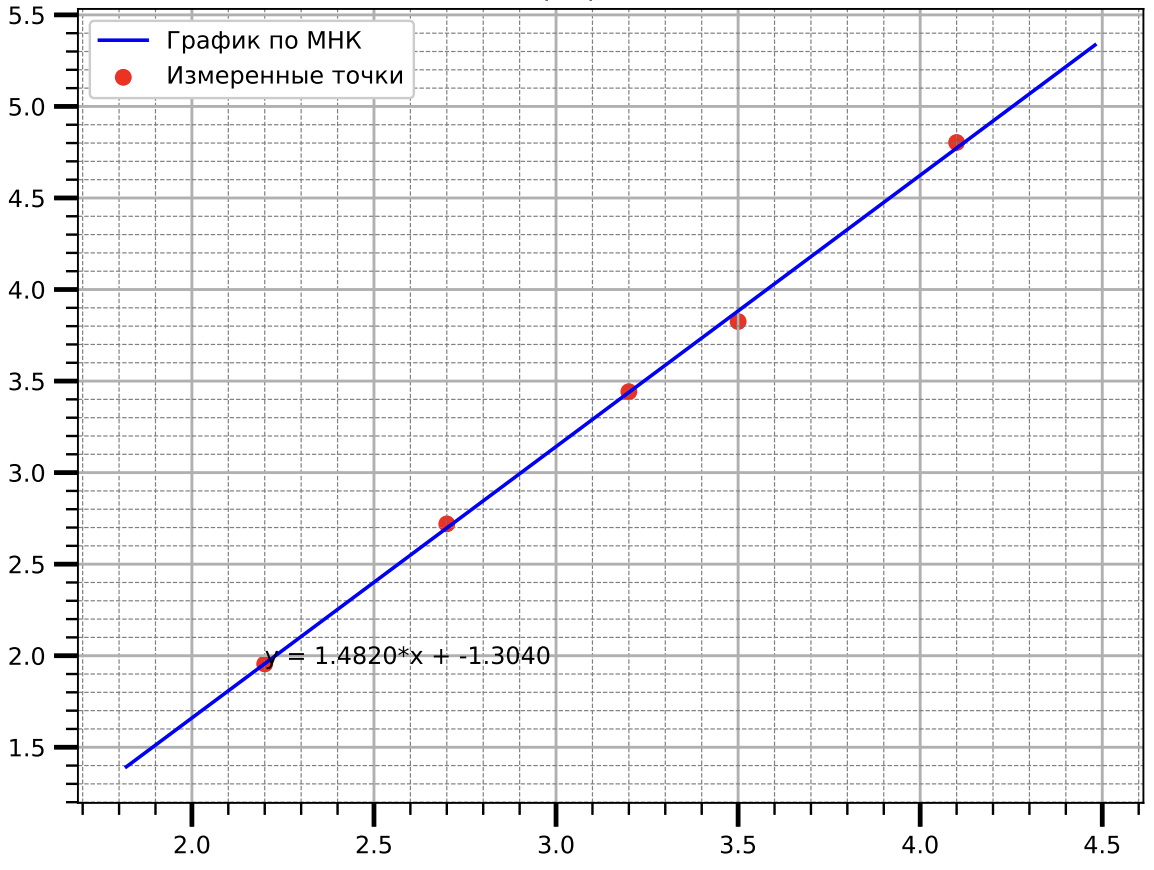
\includegraphics[width=400]{Graf4}}
	\caption{Зависимость $ \delta T / \delta P $ \ при \ T = 323 K}
\end{figure}

Получилась зависимость: 


\[ \frac{\delta T}{\delta P} = 1.5 \pm 0.5 \ \frac{K}{Па}\]

\medskip
\newpage


\\\\\\\\\\\\\\\\\\\\\\\\\\\\\\\\\\\\\\\\\\\\ 


\item Построим график $\mu$ от $\frac{1}{T}$:

$$
\begin{tabular}{|c|c|c|c|c|}
\hline
$\frac{1}{T}, 10^{ -3} K^{ -1}$&3.4&3.7&3.2&3.1\\\hline
$\mu, K/Pa$& 1.735& 1.73& 1.54& 1.482\\\hline
\end{tabular}
$$

\begin{figure}[h]
	\center{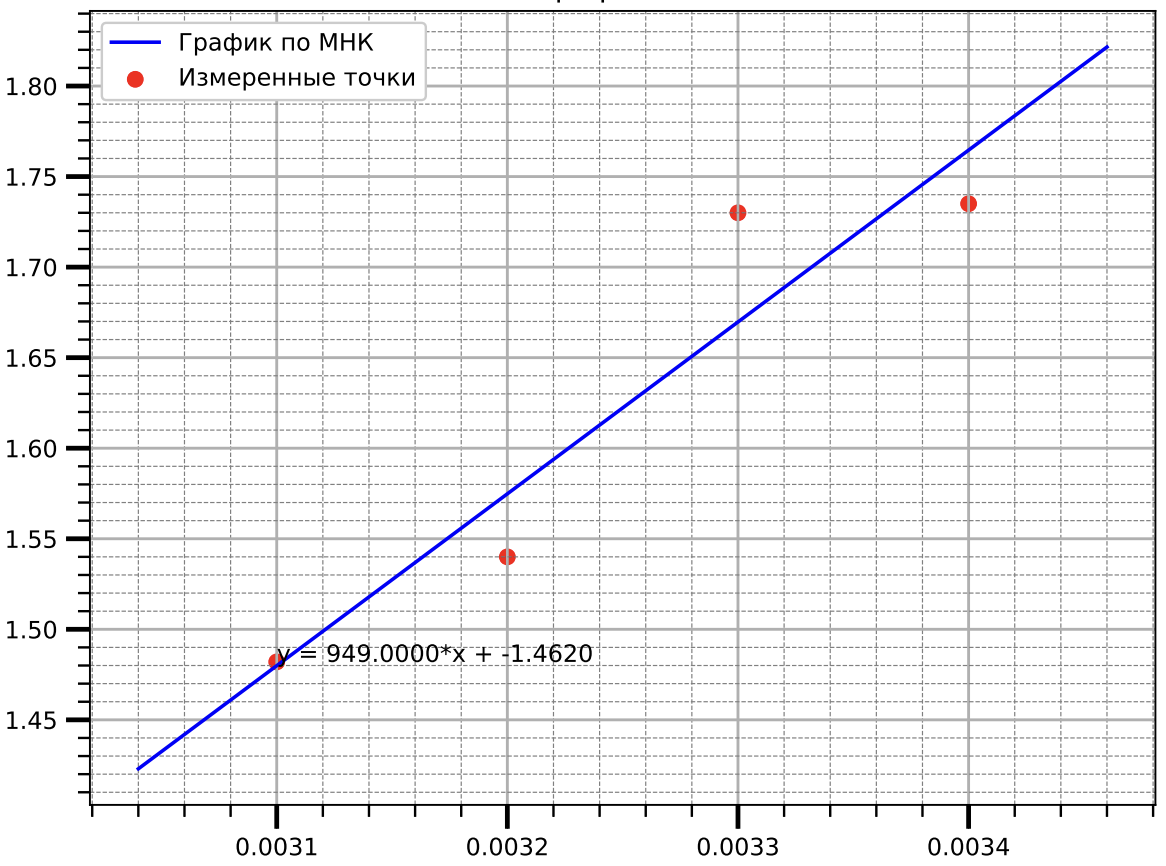
\includegraphics[width=400]{Graf5}}
	\caption{Зависимость $\mu$ от $\frac{1}{T}$}
\end{figure}

Полученная линейная зависимость: $y =  949x - 1.462$,
$\sigma_a = 0.006 K^2/Па$\\


Используя формулу $\mu = \frac{2}{RTC_p} \cdot a  -  \frac{b}{C_p}$ по коэффициентам прямой определим коэффициенты $a$ и $b$ для углекислого газа:

$$a = 1.46 \frac{H \cdot M^4}{моль^2}, b = 54.24 \frac{см^3}{моль}$$ \\

Табличные коэффициенты: 

$b = 42,8 \frac{см^3}{моль}$. Он достаточно точно совпадает с полученным. 

$a = 0.36 \frac{H \cdot м^4}{моль^2}$ Отличается более, чем в 3 раза.\\

По пересечению графиком $\mu \left(\frac{1}{T}\right)$ оси абсцисс находим значение температуры
инверсии для углекислого газа:
$$T_{inv} = 649 K$$
Табличное значение $T_{инв} = 2053К$, а это сильно отличается от полученного.\\


\end{enumerate}


\section{Выводы}
		 В ходе лабораторной работы были полученны коэфициенты газа Ван-дер-Ваальса и была вычислина $T_{инв}= 649$ К. Стабличным значением  согласуется только коэффициент b. Остальные параметры сильно отличаюся. Такая ошибка может говорить о неприменимости уравнения газа Ван-дер-Ваальса в данном случае, так как с помощью него обычно описывается качественная, а не количественная сторона вопроса.

\end{document}